\chapter{Error Analysis through Simulation}\label{ch:simulation}
% word checked.
The flight test results proved the feasibility of using the CC-EKF-SLAM
algorithm for distant object mapping. It also revealed there existed
some error in the result of the algorithm, with error of up to 30
meters for SUAS localization and up to 150 meters for most landmarks
positions. It is important to understand the cause of these errors so
that improvement on the algorithm can be made.

There are many factors affecting the accuracy in UAV localization and
landmarks mapping results, and they can be sorted into three main
categories:

\begin{enumerate}
  \item Error caused by the SLAM algorithm itself. The algorithm
  estimates landmarks coordinates through a model that describes the
  relation between the UAV and landmarks. As the model is non-linear,
  the linearization process introduces error into the result.
  \item Noise in system intrinsic parameters. The system intrinsic
  parameters include
  \begin{itemize}
    \item Camera intrinsic parameters
    \begin{itemize}
      \item Coordinate of optical center on image plane $[c_{x}, c_{y}]$
      \item Scaling factors that project landmarks in 3D world to image plane $ [f_{x}, f_{y}]$
      \item Lens distortion parameters $[k_{1}, k_{2}, p_{1}, p_{2}]$
    \end{itemize}
    \item Image resolution.
    \item Accelerometer bias % expand
  \end{itemize}
  \item Error introduced by Lucas-Kanade (LK) tracking algorithm.
  Firstly, LK tracking algorithm tracks landmarks by comparing the
  intensity of a windowed image centered at the landmark coordinate
  from one frame to another. The searching of the matching window
  terminates when the sum of squared error (SSE) on the windowed image
  is lower than a threshold set by the user, or when the number of
  iterations of the search has reached a maximum number (also set by
  user). As the scene evolves from frame to frame, the initial
  landmark appears differently as viewing distance and angle changes.
  Allowing a small SSE between matched windows is necessary to give
  tolerance for the matching. However, it could also cause the window
  to move in the neighborhood of the landmark coordinate, and
  eventually drift off, resulting in a loss of the original landmark.
  An example was shown in Figure \ref{fltfig:1_1} in Chapter
  \ref{ch:FlightResult}. Secondly, sudden intensity changes in image
  sequences could result in significant noise in the tracking. In an
  outdoor setting, intensity change can be introduced by many factors,
  such as changes of sky portion in an image, sun glare, UAV entering
  or exiting cloud shade, or the camera auto-adjusting its shutter
  speed, etc. As a reliable vision tracking algorithm is an entire
  field of research in itself, it will not be discussed further in
  this chapter.

\end{enumerate}

To better understand the impact from the noise of system intrinsic
parameters listed above, a series of simulations were performed to
examine items 1 and 2. The procedure described below simulates the
entire process of perceiving landmarks through a digital camera under
arbitrary UAV motion. The simulator first generates a 3D point cloud
ranging between 100 meters to 1500 meters from the camera (Figure
\ref{fig:simfig51}). At each frame, the coordinates of the 3D points
are transformed to the new camera frame using a simulated UAV pose,
which allows for studying the algorithm under various motions. Next,
the 3D points are projected onto the image plane using a camera model
defined by $[c_{x}, c_{y}, f_{x}, f_{y}, k_{1}, k_{2}, p_{1}, p_{2}]$,
and digitized to a resolution of choice. The camera model used by the
simulator may be different than the model used by the CC-EKF-SLAM
algorithm, which allows for injection of camera calibration errors.
The resulting coordinates of the 3D points were used directly as
measurements in the update of the EKF. The simulator does not simulate 
errors contributed by the visual tracking algorithm, and by navigation
measurements.

\begin{figure}[h]
\centering
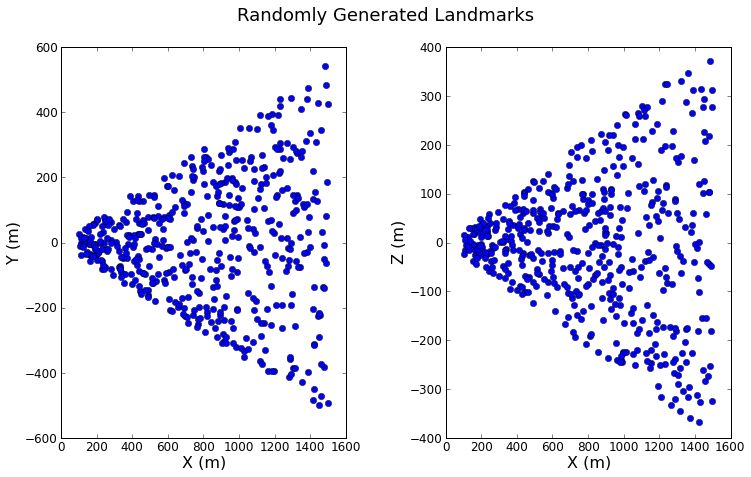
\includegraphics[width=12cm, height=7cm]{./Figures/SimulationFigures/Figure51.png}
\caption{Randomly generated 3D landmark points}
\label{fig:simfig51}
\end{figure}
\FloatBarrier

\section{An Ideal Case}
% word checked.
First of all, understanding the algorithm's performance under nearly
no noise conditions provides a solid ground for the analysis later on.
This simulation showed how much error the algorithm itself generated under
the most basic flying condition, which is moving forward at constant
speed. The low noise environment was configured as follows,

\begin{itemize}
  \item UAV was moving forward (X axis) with constant speed of 60 knots. 
  \item Y axis and Z axis translation were limited to white noise with
  standard deviation of 0.08 meters and a mean of 0.
  \item UAV rotations on all three axes were modelled by white noise with standard
  deviation of 0.01 degree and a mean of 0 degree.
  \item No image digitization error was introduced (i.e. the projected
  landmark position on the image plane was not digitized to any sensor
  resolution).
  \item No error was introduced from camera model mismatch (i.e.
  camera intrinsic parameters used by the simulator was exactly the
  same as those used in CC-EKF-SLAM algorithm).
\end{itemize}

\subsection{UAV Localization}
% word checked.
Acuracy of UAV poses estimates are plotted in Figure
\ref{fig:simfig1}. The ground truth and estimated value are plotted
in blue and green lines respectively. The error is plotted in red
line. Under a simple forward motion, the algorithm tracks the
UAV status quite well. Error on translational motion is less than 1
cm and error on rotational motion less than 3e-3 degree. An obvious
behavior of the error is that the error starts from 0, experiences
some rapid change during the first few frames, and settles to a
relatively stable value. This matches the converging behavior of the
landmark inverse depth $\rho$ which was shown next. This observation
suggests that although the inverse depth representation is more linear
than th direct depth representation, it has a negative impact on the
accuracy of the estimates when being included in the filter vector
before its approximate value is known. Hence, delaying integration of
inverse depth till its value is approximately known should increase
the accuracy of the state vector estimates. As triangulating a
landmark requires 2 frames in a monocular vision setup, the delay
requires only one extra frame, and is insignificant in most scenarios.

\begin{figure}[h]
\centering
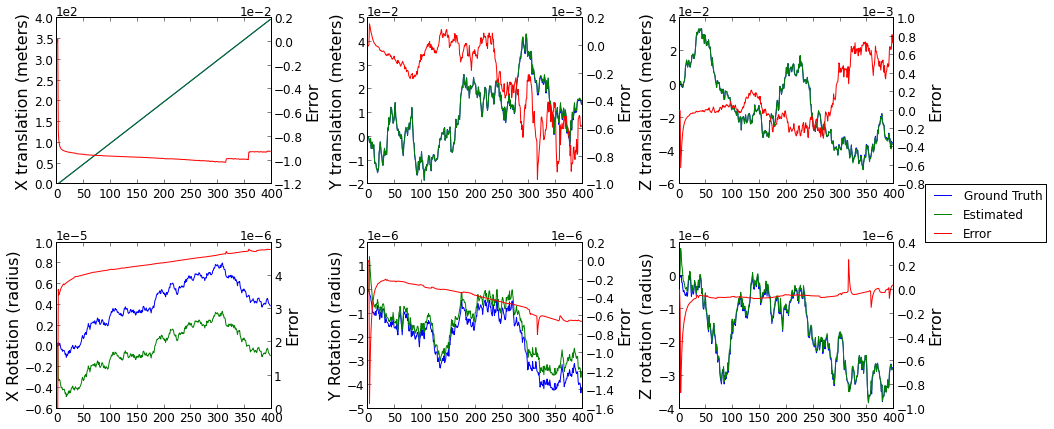
\includegraphics[width=16cm, height=8cm]{./Figures/SimulationFigures/Figure1.png}
\caption{UAV localization errors under low noise condition and forward motion}
\label{fig:simfig1}
\end{figure}
\FloatBarrier

\subsection{Landmarks Mapping}
% word checked.
Figure \ref{fig:simfig5-8} top left shows landmark parameters $[d,
\varphi ,\theta]$ (where $d=1/\rho $) plotted against frame number for
the first 50 frames. The landmark depth $d$ for all landmarks
converges within the first 3 frames. The elevation-azimuth angles
$[\varphi ,\theta]$ stay almost constant after initialization. More
detail can be seen from the error convergence plot for these
parameters, plotted in Figure \ref{fig:simfig5-8} top right. The error
of landmark distance $d$ slowly converges to zero. $[\varphi ,\theta]$
errors starts from 0 at frame 0, and converge to a small offset
while landmark depth $d$ converge. As discussed in Chapter
\ref{ch:FlightResult}, in order to compensate for the inaccurate
estimates of depth at filter initialization, the EKF makes adjustments
to $\varphi$ and $\theta$ so that the resulting coordinates of
landmarks agree with the measurements. Therefore early integration of
landmark depth also has negative impact on the accuracy of landmarks
positions estimation.

\begin{figure}[h]
\centering
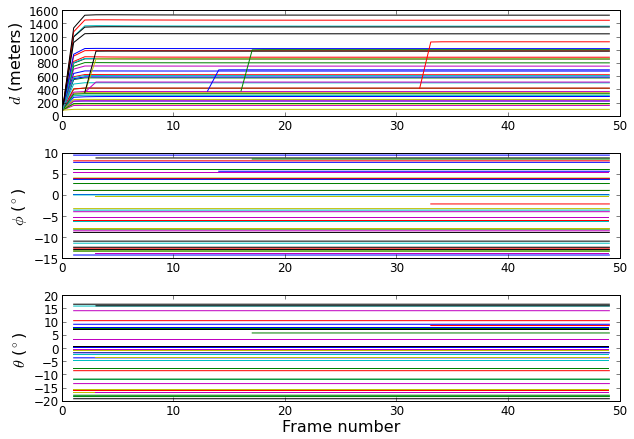
\includegraphics[width=7cm, height=5cm]{./Figures/SimulationFigures/Figure6.png}
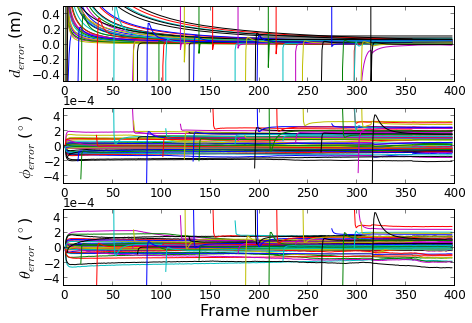
\includegraphics[width=7cm, height=5cm]{./Figures/SimulationFigures/Figure7.png}
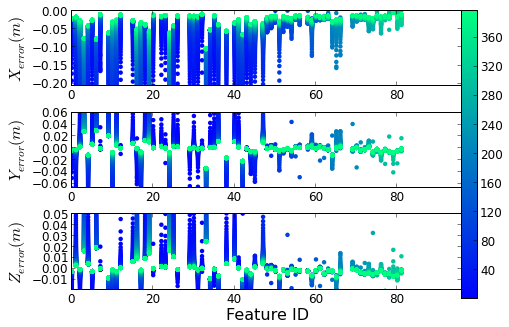
\includegraphics[width=7cm, height=5cm]{./Figures/SimulationFigures/Figure5.png}
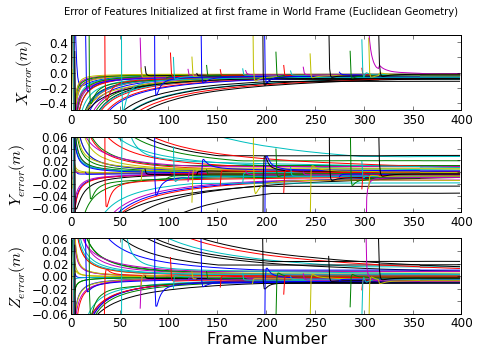
\includegraphics[width=7cm, height=5cm]{./Figures/SimulationFigures/Figure8.png}
\caption{Landmark parameters and errors convergence under low noise
  condition and forward motion}
\label{fig:simfig5-8}
\end{figure}

The errors for landmark coordinates in world frame are plotted
against landmarks IDs and frame number in Figure \ref{fig:simfig5-8}
bottom left and right. The landmark coordinate errors in world frame
all converge toward zero. During the 400 frames period, some
landmarks move out of the FOV, and therefore their position estimates
remain unchanged afterward. At the end of the 400 frames, landmark
coordinate errors on X axis are reduced to +/-0.2 meters; on Y and Z axes,
errors are reduced to +/-0.02 meters. In summary, factors that cause
error in landmark positions are listed below. 

\begin{itemize}
  \item Errors in UAV localization cause an offset error when a new
  landmark is added to the filter.
  \item Early landmark integration causes offset errors in $\varphi$
  and $\theta$ estimates due to the EKF compensating for landmark depth at
  integration.
  \item Some landmarks move out of FOV before fully converged.
\end{itemize}
\FloatBarrier

\section{Effect of UAV Oscillatory Motion}
% word checked.
The simulation of UAV forward travel shows that the
CC-EKF-SLAM algorithm does landmark tracking and self localization
quite well under simple motion. Next, the algorithm was tested with a
more complex and realistic scenario. The remaining 5 types of
maneuvers were examined independently. These maneuvers are:
translation on Y, translation on Z, rotation on X, rotation on Y and
rotation on Z. As motions on all other 5 DOFs are mostly oscillatory
when the UAV moves forward, each motion was modelled by a Sine wave
with frequency at 1Hz and variable amplitude.

$$\text{Added motion} = A_{\text{motion type}}\cdot sin(2\pi x+\pi/2)$$

Motion type is denoted by $v_y$, $v_z$ for translation on Y and Z
axes; $w_x$, $w_y$ and $w_z$ for rotation on X, Y, and Z axes. For
translation, the Sine amplitude $A_{v_y,v_z}$ varied from 1 meter to
19 meters with 2 meter increments. For rotation, the amplitude
$A_{w_x,w_y,w_z}$ varied from 0.001 radians to 0.018 radians
(0.057$^\circ$ to 1.031$^\circ$) with 0.001 radian increments.

\subsection{UAV Localization}\label{localization_motion}

Figure \ref{fig:simfig9-10} shows the UAV localization error statistic
under oscillatory translation on Y and Z axes and oscillatory rotation
on X, Y, and Z axes. The blue dots marks the mean value $\mu$ of the
error averaged throughout 400 frames of tracking, and the error bars
marks the standard deviation $\sigma$.

The translation motion clearly increases the error of UAV
localization. However, the amount is insignificant. With the Sine
amplitude increased to 19m, the UAV position error increases by less than
0.02 meter.

On the other hand, rotational motions have a big impact on the accuracy
of localization. Rotations around the X axis (roll) have small effect. No
obvious increase in mean and standard deviation can be
observed. Rotations around Y and Z axes yield significant errors.

\begin{itemize}
  \item Rotation around the Y axis increases the mean and standard deviation
  of UAV position error on X. For UAV position on Z, the mean
  error stays zero, but standard deviation increases dramatically.
  \item The same behavior can be observed on the X and Y axes position
  error for rotation around the Z axis.
\end{itemize}

\begin{figure}[h]
  \centering
  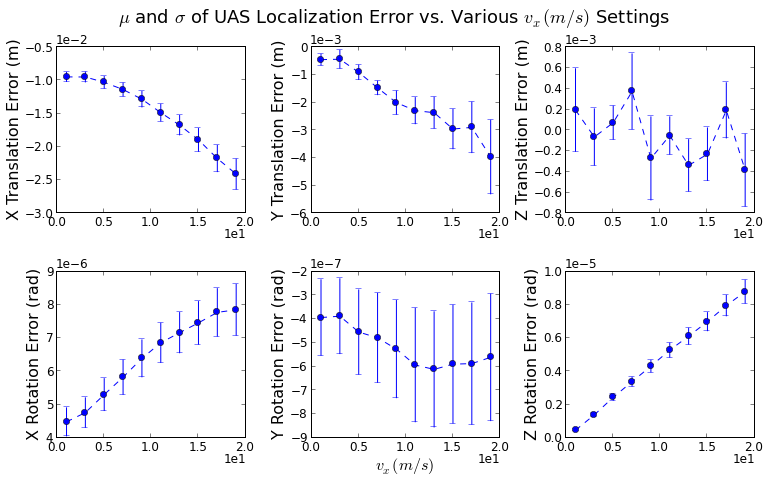
\includegraphics[width=7cm, keepaspectratio=true]{./Figures/SimulationFigures/Figure9.png}
  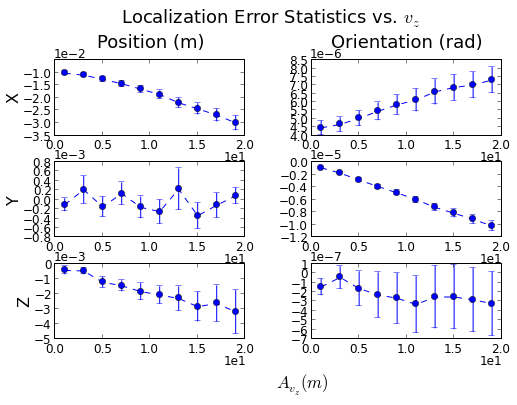
\includegraphics[width=7cm, keepaspectratio=true]{./Figures/SimulationFigures/Figure10.png}
  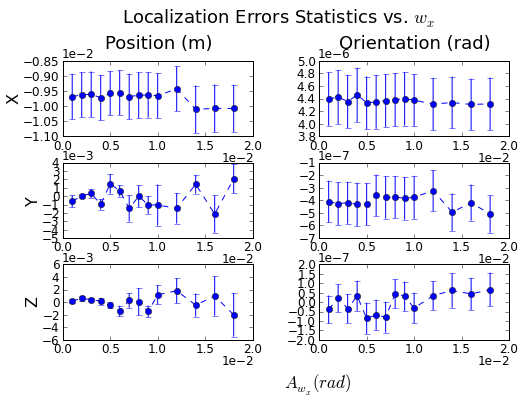
\includegraphics[width=7cm, keepaspectratio=true]{./Figures/SimulationFigures/Figure11.png}
  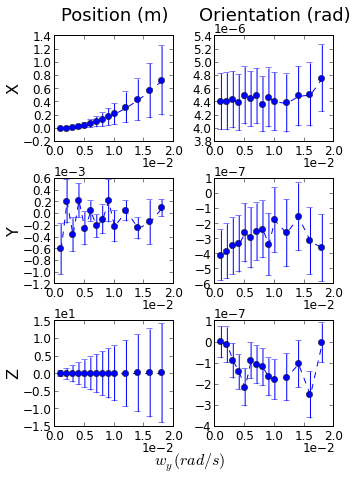
\includegraphics[width=7cm, keepaspectratio=true]{./Figures/SimulationFigures/Figure12.png}
  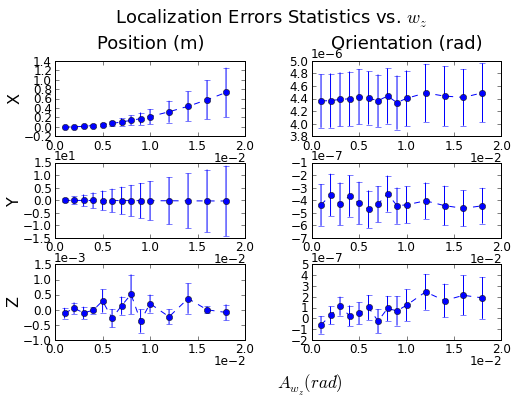
\includegraphics[width=7cm, keepaspectratio=true]{./Figures/SimulationFigures/Figure13.png}
  \caption{UAV localization error statistics under oscillatory motion} 
  \label{fig:simfig9-10}
\end{figure}
\FloatBarrier

To understand how rotation affects the UAV localization estimates,
UAV position errors in world frame are plotted below (Figure
\ref{fig:simfig14}) with $A_{w_x,w_y,w_z}$ set to
0.01 radians. When rotation occurs around the X axis, the position error of
the UAV shows some oscillation on Y and Z axes. The oscillation
magnitude remains small (on the scale of millimeters) and around
zero. Hence, it does not generate significant mean and standard deviation
change on the error statistic plot. For rotation around Y and Z, increase
of rotational motion causes an increasing oscillatory error on the UAV
position estimates (diverging). The mean UAV position error on the X axis
increases in positive direction with rotation around both Y and Z
axes. The most significant impact happens on the Z axis position (for
rotation around Y) and Y axis position (for rotation around Z), with errors
reaching 20 meters peak-to-peak at the end of the 400 frames. With an
increasing rate of rotation, the rate of
error diverging from zero also increases, and results in an
increasing error standard deviation in the error statistic plots. This
result suggests that the CC-EKF-SLAM algorithm is very
sensitive to rotational motion around Y and Z axes.

\begin{figure}[h]
  \centering
  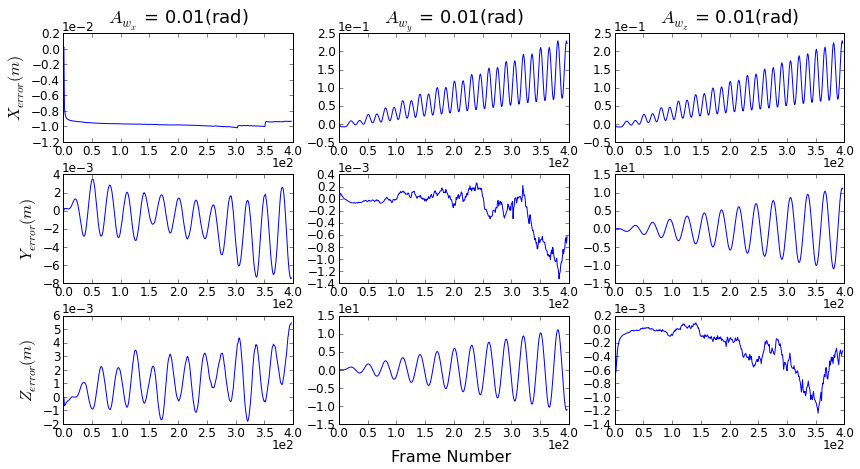
\includegraphics[width=13cm, keepaspectratio=true]{./Figures/SimulationFigures/Figure14.png}
  \caption{Estimated UAV position in world frame with oscillatory
    rotation, $A_{w_x,w_y,w_z} = 0.01 rad$}
  \label{fig:simfig14}
\end{figure}
\FloatBarrier

\subsection{Landmark Mapping}\label{sec:landmarkMotion}
% word checked.
Landmark mapping error statistics were calculated from the landmark
errors at the last frame. Figure \ref{fig:simfig20-24} shows the
landmark mapping error statistics with added motions. 

Translational motions increase both the mean and standard deviation
of landmark mapping errors, but not by much. With $A_{v_x, v_y}$
ranging from 1 meter to 19 meters, the increases in mean and standard
deviation are both on the scale of centimeters.

\begin{figure}[h]
  \centering
  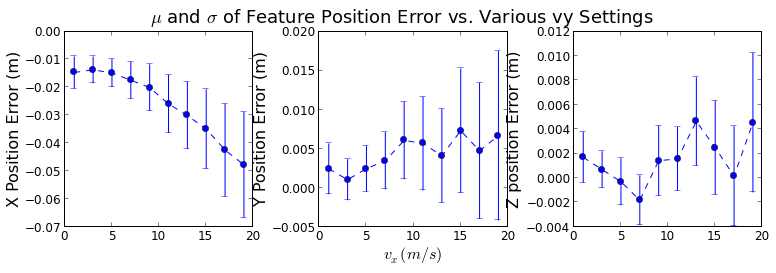
\includegraphics[width=10cm, keepaspectratio=true]{./Figures/SimulationFigures/Figure20.png}
  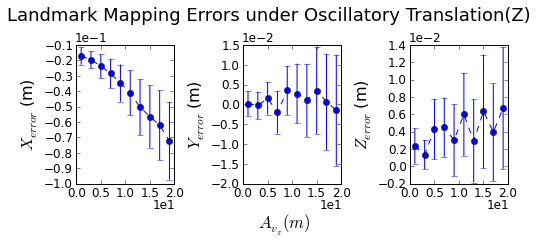
\includegraphics[width=10cm, keepaspectratio=true]{./Figures/SimulationFigures/Figure21.png}
  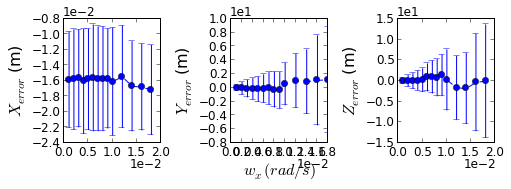
\includegraphics[width=10cm, keepaspectratio=true]{./Figures/SimulationFigures/Figure22.png}
  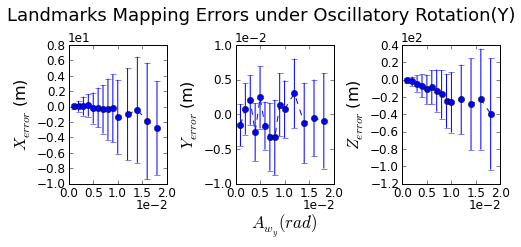
\includegraphics[width=10cm, keepaspectratio=true]{./Figures/SimulationFigures/Figure23.png}
  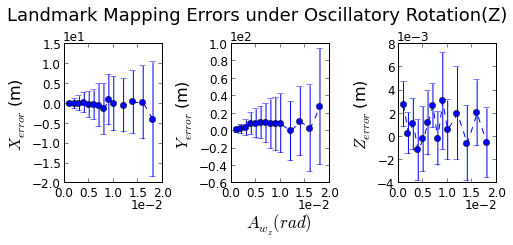
\includegraphics[width=10cm, keepaspectratio=true]{./Figures/SimulationFigures/Figure24.png}
  \caption{Landmark mapping error statistics under oscillatory motion}
  \label{fig:simfig20-24}
\end{figure}

Rotational motion has much bigger effect on the accuracy. With
$A_{w_x, w_y, w_z}$ ranging from 0.001 radians to 0.018
radians (0.057$^\circ$ to 1.031$^\circ$)

\begin{itemize}
  \item Rotation around the X axis causes a small standard deviation
  increase in the errors of landmark positions on the Y and Z axes.
  The errors are on the scale of meters under the maximum rotation
  setting.
  \item Rotation around the Y axis causes mean and standard deviation
  increase in landmark position errors on the X and Z axes. Landmark
  positions on Z receive the biggest impact with errors on the scale
  of hundreds of meters under the maximum rotation setting.
  \item Rotation around the Z axis affects landmark mapping on X and Y
  axes in a similar way as the Y axis rotation does.
\end{itemize}
\FloatBarrier
\begin{figure}[h]
  \centering
  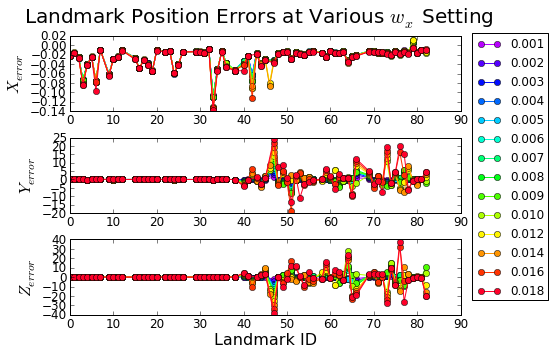
\includegraphics[width=7cm, height=5cm]{./Figures/SimulationFigures/Figure17.png}
  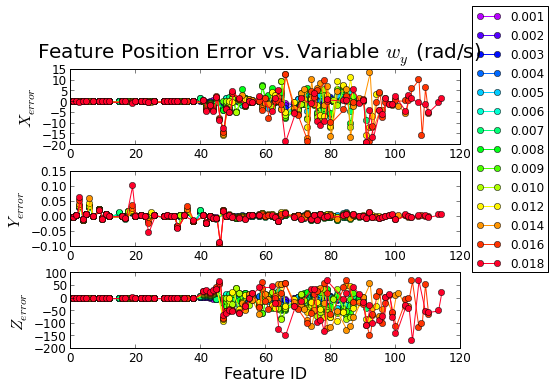
\includegraphics[width=7cm, height=5cm]{./Figures/SimulationFigures/Figure18.png}
  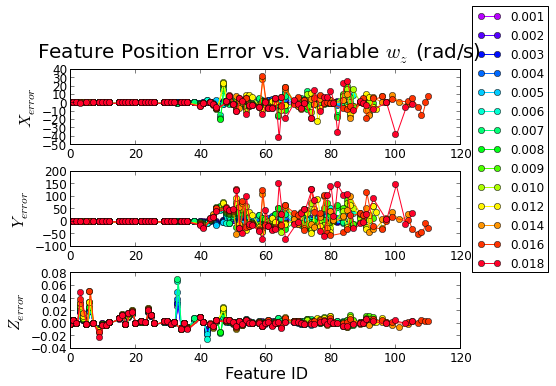
\includegraphics[width=7cm, height=5cm]{./Figures/SimulationFigures/Figure19.png}
  \caption{Landmark mapping errors plotted against initialization sequence under oscillatory rotation}
  \label{fig:simfig17-19}
\end{figure}

Figure \ref{fig:simfig17-19} shows landmark position errors at
the last frame plotted against landmark IDs (initialization
sequence), with line and marker color indicating rotation amplitude
setting. The following observations can be made from the plots:

\begin{itemize}
  \item With rotation around Y and Z, tracked landmarks were easily lost
  as they move out of the FOV. This can be observed from the increase of
  landmark IDs when Y axis rotation setting is increased from 0.001rad to
  0.018rad. A frequent addition of new landmarks has a negative impact on
  the overall result due to the correlation between landmarks.
  \item Landmarks added after first frame have a much bigger error than
  landmarks added at the first frame. At the first frame, 40 landmarks were
  added to the filter. All three plots in Figure \ref{fig:simfig17-19}
  show that major landmark mapping errors come from landmarks added
  after the first frame with ID bigger than 40.
\end{itemize}
\FloatBarrier

To investigate how oscillatory rotations resulted in bigger error for
landmarks added after the first frame, the scenario of UAV
experiencing rotation around the Y axis with $A_{w_y}=0.01rad$ was
analyzed. Landmark parameters were converted into the world frame and
their errors are shown in Figure \ref{fig:simfig25}. It was found that
the most significant error occurs on parameter $\varphi$ which is the
landmark elevation angle. This angle has the same definition as the
rotation angle around the Y axis. The second biggest error contributor
is $z_i$, the landmark initialization coordinate on Z axis. Both
parameters $\varphi$ and $z_i$ had an offset error at initialization, and
were never corrected by the filter throughout the tracking.

Regarding the offset error in $z_i$, as discussed in Section
\ref{localization_motion}, UAV localization estimates have the biggest
position error on the X and Z axes under Y axis rotation. All landmarks
not initialized at the first frame are affected by the UAV
localization error, since the initialization point and UAV position
are correlated.

\begin{figure}[h]
  \centering
  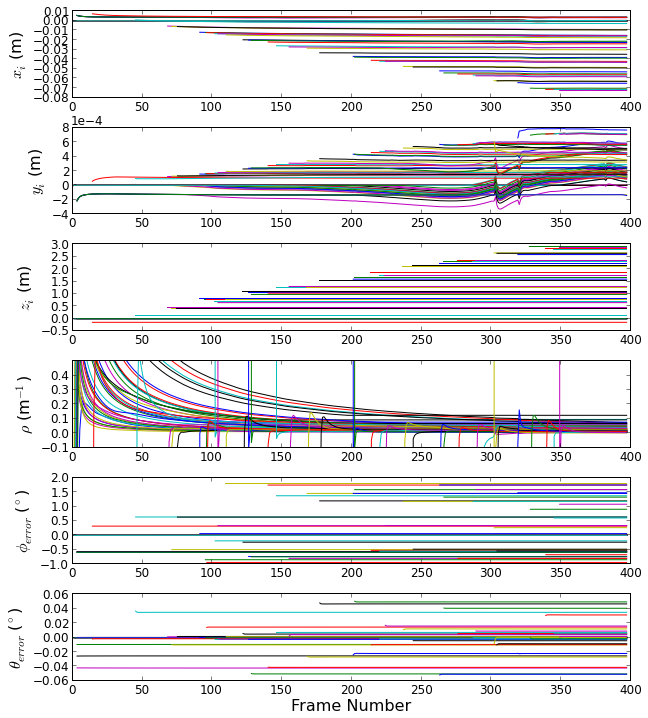
\includegraphics[width=10cm, height=12cm]{./Figures/SimulationFigures/Figure25.png}
  \caption{Landmark parameter errors under
    oscillatory rotation around the Y-axis, $A_{w_y}=0.01rad$}
  \label{fig:simfig25}
\end{figure}
\FloatBarrier

Figure \ref{fig:simfig26} shows the $\varphi$ error at initialization
in the camera frame and the world frame. The blue line shows the error in
camera frame. The red line shows the error in world frame. As
$\varphi$ error is nearly 0 in the camera frame, it is clear that the
reference frame transformation from camera frame to world frame
introduced the offset error. During reference frame transformation,
ground truth landmarks are transformed using the ground truth UAV
poses; estimated landmarks are transformed using estimated UAV poses.
Hence, even though the parameters are the same in the camera frame,
results in the world frame are different. Landmarks initialized at the
first frame do not carry any offset error because the reference frame
transformation uses the same parameters in both ways. During
tracking, these landmarks are transformed to the new camera frame
using the estimated UAV position and orientation. These are the same
values being used to transform landmark positions from the camera frame
back into the world frame. Therefore, although the UAV localization
estimates are different from the ground truth, landmarks initialized
at the first frame are not affected.

To conclude, the main contributor for landmark mapping errors come
from errors in UAV localization estimation.

\begin{figure}[h] %redo figure, change phi to varphi
  \centering
  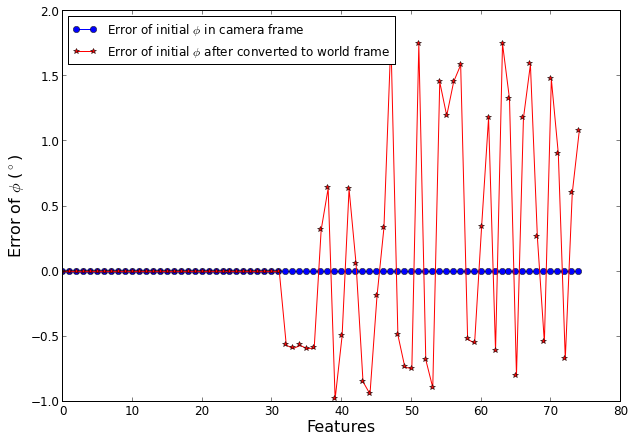
\includegraphics[width=10cm, height=7cm]{./Figures/SimulationFigures/Figure26.png}
  \caption{Error of $\varphi$ at initialization in camera frame and
    world frame}
  \label{fig:simfig26}
\end{figure}
\FloatBarrier

\section{Effect of Errors in Camera Intrinsic Parameters}
% word checked.
This section discusses the effect on CC-EKF-SLAM accuracy from
calibration errors of camera intrinsic parameters. Errors in camera
intrinsic parameters were simulated by using different 
camera models in the simulator and in CC-EKF-SLAM algorithm.
$c_{x}$, $c_{y}$, $f_{x}$, and $f_{y}$ were simulated individually and
distortion parameters $[k1, k2, p1, p2]$ were simulated as a group.
Using the calibration result (see Section \ref{sec:camcal}) as a
base model, $c_{x}$, $c_{y}$, $f_{x}$, and $f_{y}$ in the simulator
varied from -50\% to 50\% of the base model. Distortion
parameters varied from 0\% to 140\% of the base model.

\subsection{Effect of Errors in $(c_{x}, c_{y})$}
% word checked.
Figure \ref{fig:simfig34-35} shows an overview of UAV pose error
statistics with calibration error introduced into $(c_{x}, c_{y})$. From
the statistic plot, it was found that $c_x$ had the biggest impact on UAV
position on X and Y, and $c_y$ had the biggest impact on UAV position on X
and Z.

\begin{figure}[h]
  \centering
  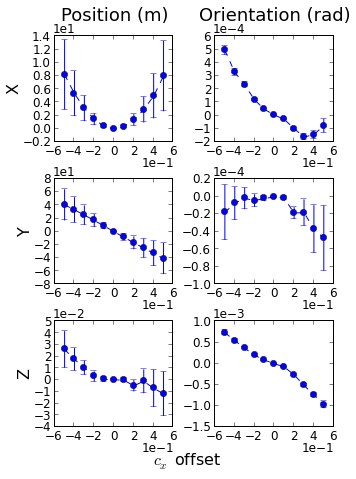
\includegraphics[width=7cm, keepaspectratio=true]{./Figures/SimulationFigures/Figure34.png}
  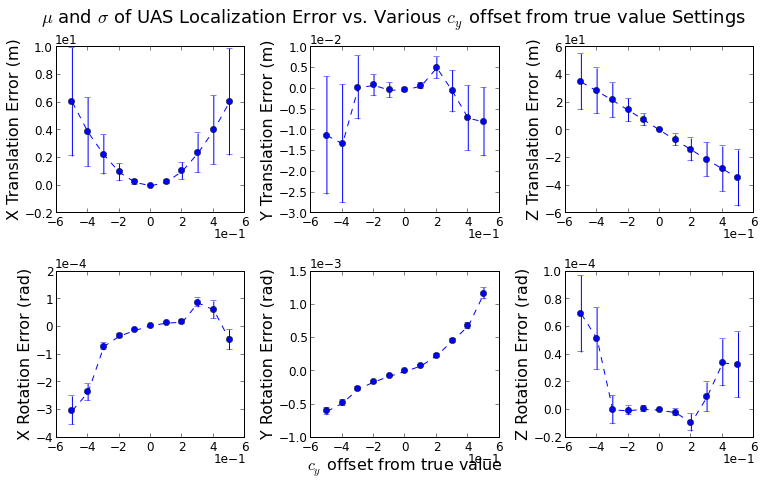
\includegraphics[width=7cm, keepaspectratio=true]{./Figures/SimulationFigures/Figure35.png}
  \caption{UAV localization error statistics with various $(c_x, c_y)$
  settings}
  \label{fig:simfig34-35}
\end{figure}

Figure \ref{fig:simfig36-37} shows the UAV position errors with $c_x$
and $c_y$ at various offsets from the base value. The resulting UAV
position errors are dependent on $(c_{x}, c_{y})$ and are
divergent in time. The divergence can be modeled by a first order
polynomial function, with the rate of divergence decided by the offset
of $(c_{x}, c_{y})$ from the base value.

\begin{figure}[h]
  \centering
  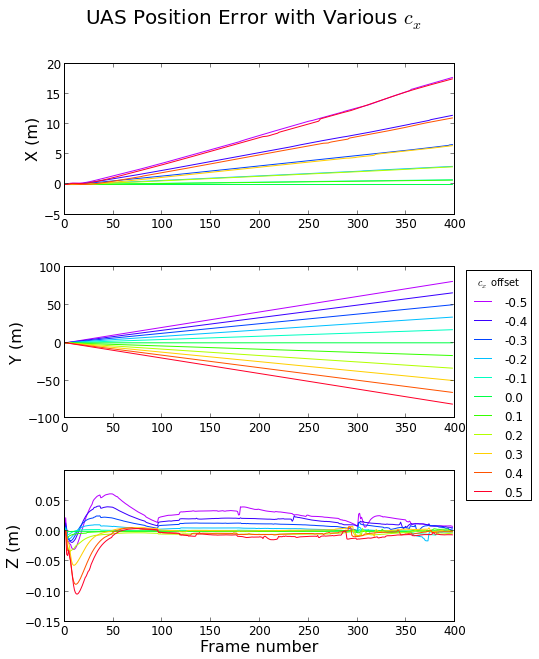
\includegraphics[width=7cm,keepaspectratio=true]{./Figures/SimulationFigures/Figure36.png}
  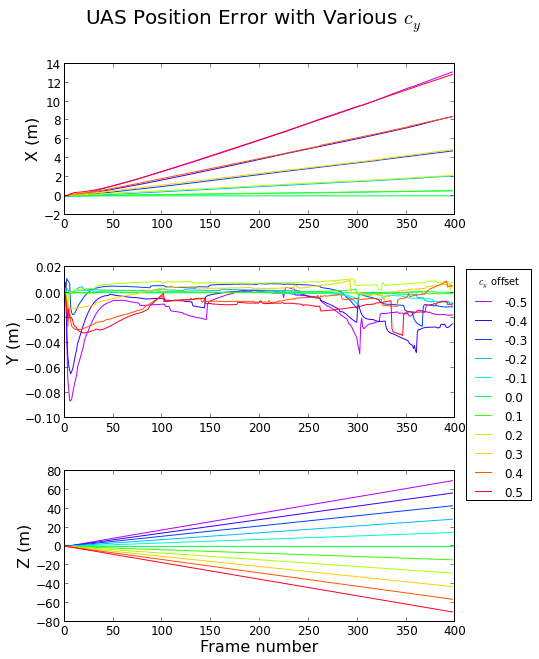
\includegraphics[width=7cm,keepaspectratio=true]{./Figures/SimulationFigures/Figure37.png}
  \caption{Diverging UAV position errors with error in$(c_x, c_y)$ }
  \label{fig:simfig36-37}
\end{figure}
\FloatBarrier

The statistics of the landmark mapping errors due to the calibration errors of
$(c_{x}, c_{y})$ are plotted in Figure \ref{fig:simfig28-29}. The
following characteristics can be observed from the plots:

\begin{itemize}
  \item Calibration error in $c_{x}$ affects landmark positions on all
  axes, among which, the X and Y axes show the most significant error.
  \begin{itemize}
    \item The further $c_{x}$ deviates from the base value, the further
    the landmarks appear on average (positive mean error on X).
    \item Mean landmark position errors on the Y axis are proportional to
    the calibration error in $c_x$. Their relation can be modeled by a
    first order polynomial equation.
    \item Error in $c_{x}$ also affects landmark positions on the Z
    axis, but on the scale of a few meters.
  \end{itemize}
  \item Calibration error in $c_{y}$ affects landmark positions on
  all axes similarly to $c_{x}$. Estimates on the X and Z axes show the
  greatest amount of error.
\end{itemize}

\begin{figure}[h] % change plots title to "Landmarks Mapping Errors
                  % Statistics
                  % and C_x/C_y offset
  \centering
  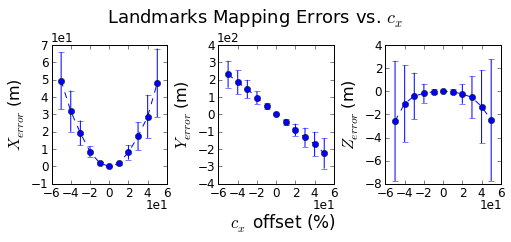
\includegraphics[width=10cm, keepaspectratio=true]{./Figures/SimulationFigures/Figure28.png}
  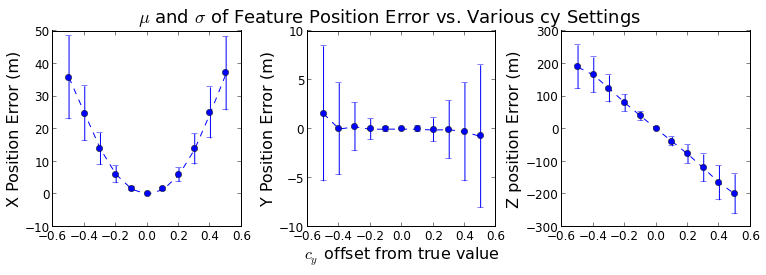
\includegraphics[width=10cm, keepaspectratio=true]{./Figures/SimulationFigures/Figure29.png}
  \caption{Landmark mapping error statistics with various $(c_x, c_y)$
  settings}
  \label{fig:simfig28-29}
\end{figure}

Plotting landmark position errors against landmark ground truth
positions reveals more information on how $c_{x}$ and $c_{y}$
affects landmark mapping. Landmark position errors are dependent
on their ground truth positions, and the amount of error in $c_{x}$
(or $c_{y}$).

\begin{itemize}
  \item Landmark position errors on the X axis are proportional to the
  landmarks ground truth positions on X. The further the landmark is,
  the greater the error. The amount of error in $c_{x}$
  determines the slope of the error plot. The greater the error is in
  $c_{x}$, the steeper the slope becomes (Figure \ref{fig:simfig32-33},
  top plot, subplot $[1,1]$).
  \item Landmark position errors on the Y axis are also proportional to
  their ground truth positions on X with the slope steepness and
  polarity dependent on the amount and polarity of the error in
  $c_{x}$ (Figure \ref{fig:simfig32-33}, top plot, subplot $[2,1]$).
  \item Landmark position errors on the Z axis are proportional to
  their ground truth positions on Z, with slope steepness and polarity
  dependent on the amount and polarity of error in $c_{x}$ (Figure
  \ref{fig:simfig32-33}, top plot, subplot $[3,3]$).
  \item Error in $c_{y}$ affects landmark positions similarly to
  $c_{x}$, but on different axis (Figure \ref{fig:simfig32-33}, bottom
  plot).
\end{itemize}

\begin{figure}[h]
  \centering
  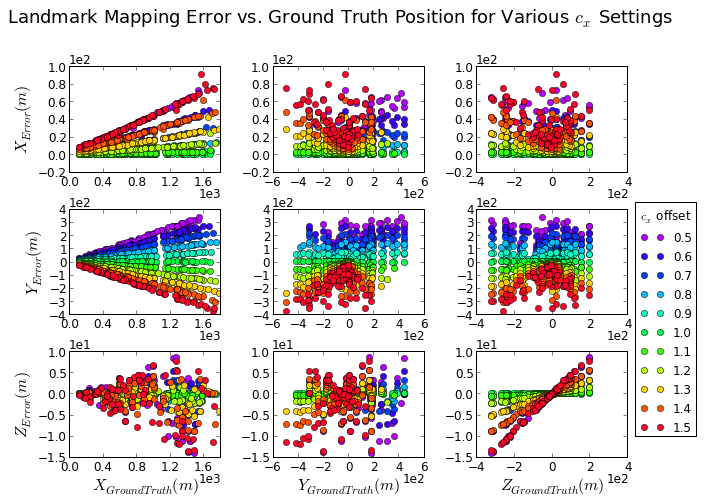
\includegraphics[width=13cm, keepaspectratio=true]{./Figures/SimulationFigures/Figure32.png}
  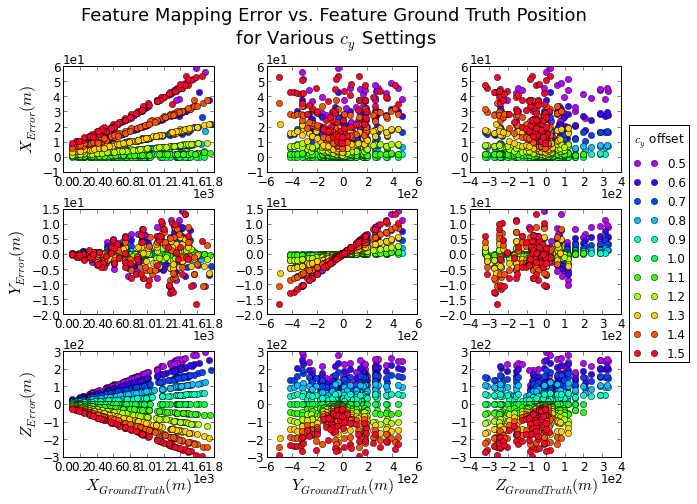
\includegraphics[width=13cm, keepaspectratio=true]{./Figures/SimulationFigures/Figure33.png}
  \caption{Landmark mapping errors versus ground truth
    landmark positions for various $(c_x, c_y)$ settings}
  \label{fig:simfig32-33}
\end{figure}
\FloatBarrier

\subsection{Effect of Errors in $(f_x, f_y)$}

With $(f_x, f_y)$ varying from -50\% to +50\% of the base value, the
UAV localization errors are shown in \ref{fig:simfig43-44}. For all
$f_x$ and $f_y$ settings, UAV position errors remain less than
+/-0.05 meters, and orientation errors remains less than 8e-6 radius.
Compared to the errors obtained from the ideal case, calibration
errors in $(f_x, f_y)$ introduce minor errors into UAV localization
estimates.
\begin{figure}[h]
  \centering
  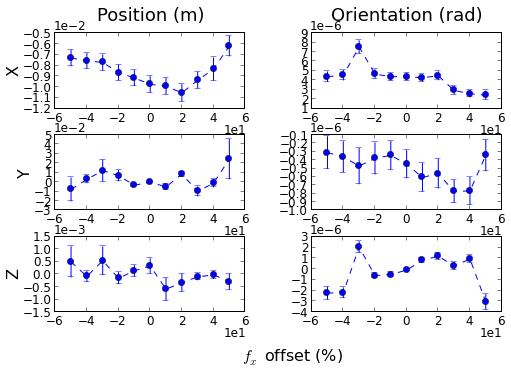
\includegraphics[width=7cm,keepaspectratio=true]{./Figures/SimulationFigures/Figure43.png}
  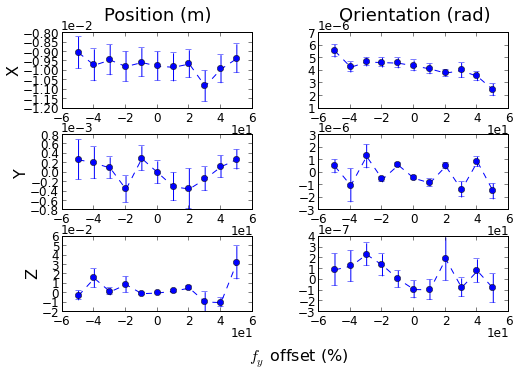
\includegraphics[width=7cm,keepaspectratio=true]{./Figures/SimulationFigures/Figure44.png}
  \caption{UAV localization error statistics with various $(f_x, f_y)$
  settings}
  \label{fig:simfig43-44}
\end{figure}

On the other hand, landmark mapping errors are unavoidably affected by
the calibration errors in $(f_x, f_y)$ since these are the scaling
factors that project landmarks from the 3D world onto the image plane.
Figure \ref{fig:simfig38-39} shows the error statistics of landmark
position estimates under various $(f_x, f_y)$ settings. The error on
the X axis is minimal and is on the scale of millimeters. Errors on
the Y axis receive the most impact from error in $f_x$, since this is
the scaling factor that maps the Y component of landmark position in
the world frame onto the u-axis on the image plane by $u = Y/X \cdot
f_x$. The same behavior happens on the landmark position estimates on
the Z axis and its relation to $f_y$.

\begin{figure}[h]% Change title to "Landmarks mapping Errors
                 % Statistics and Projection Scalling Factor (f_x/f_y)
  \centering
  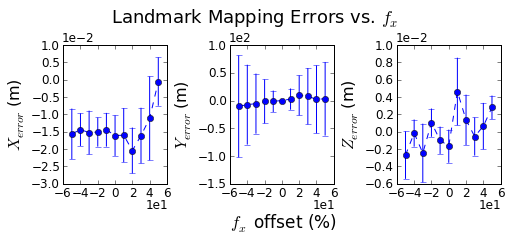
\includegraphics[width=10cm,keepaspectratio=true]{./Figures/SimulationFigures/Figure38.png}
  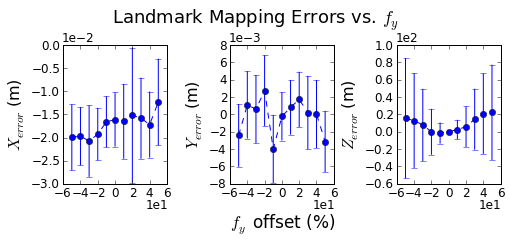
\includegraphics[width=10cm,keepaspectratio=true]{./Figures/SimulationFigures/Figure39.png}
  \caption{Landmark mapping error statistics with various $(f_x, f_y)$
  settings}
  \label{fig:simfig38-39}
\end{figure}

Plotting the landmark mapping errors against landmark ground truth
positions also indicates that the mapping errors are dependent on
landmark ground truth positions and error in $(f_x, f_y)$. When $f_x$
contains errors, landmark position errors on Y are directly
proportional to the Y component of their ground truth positions, with the
error in $f_x$ determining the steepness of the slope. The same relation can be
found for $Z_{error}$ with $f_y$, and $Z_{\text{ground truth}}$.

\begin{figure}[h]
  \centering
  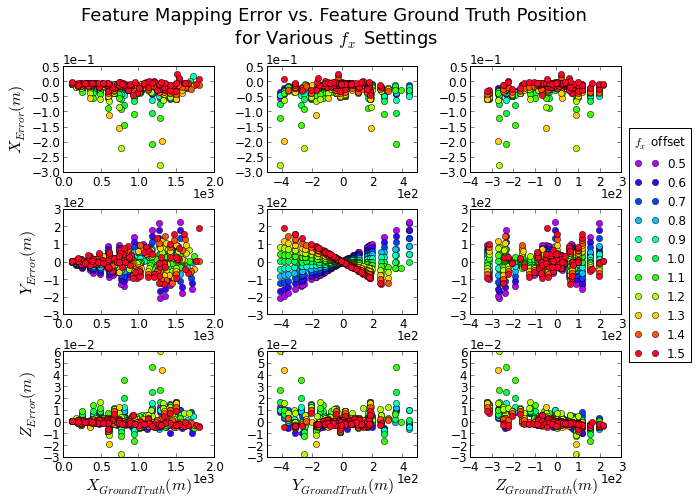
\includegraphics[width=13cm,keepaspectratio=true]{./Figures/SimulationFigures/Figure41.png}
  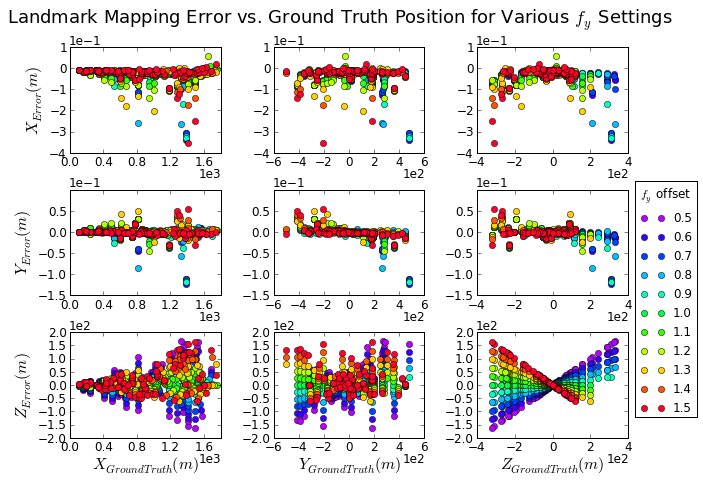
\includegraphics[width=13cm,keepaspectratio=true]{./Figures/SimulationFigures/Figure42.png}
  \caption{Landmark mapping errors versus ground truth
    landmark positions for various $(f_x, f_y)$ settings}
  \label{fig:simfig41-42}
\end{figure}
\FloatBarrier

\subsection{Effect of Errors in Distortion Model}
% word checked.
The CC-EKF-SLAM algorithm does not consider camera lens distortion
at this stage. Therefore, the simulation evaluated the effect of
lens distortion varying from 0\% to 150\% of the base value to
estimate the amount of error resulting from ignoring the lens distortion.

Figure \ref{fig:simfig47} shows the UAV localization error for
various lens distortion settings. Ignoring the distortion brings
significant error into the UAV localization. UAV position on the X axis
receives the most impact. The errors are up to 100 meters, and have
increasing standard deviation. Positions on the Y and Z axes show less
error, but standard deviation grows larger with the increasing amount of
distortion added. 

Figure \ref{fig:simfig48} reveals the cause of increasing standard
deviation. UAV position errors are diverging in time and with the amount
of lens distortion added. UAV orientation errors increase from
maximum mean error of 5e-6 rad in low noise simulation to 2.5e-4
rad. Similar to position error, the plots of orientation error vs.
frame number shows that the error amplitude increases with time
but fluctuates around zero.

\begin{figure}[h]
  \centering
  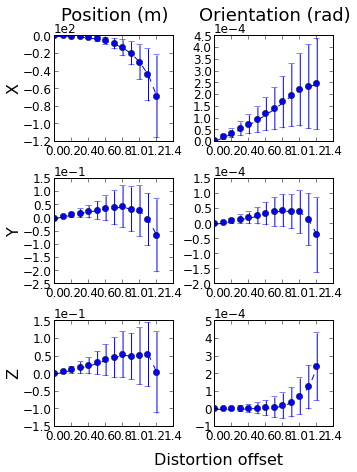
\includegraphics[width=10cm,keepaspectratio=true]{./Figures/SimulationFigures/Figure47.png}
  \caption{UAV localization error statistics with various lens
    distortion setting}
  \label{fig:simfig47}
\end{figure}

\begin{figure}[h]
  \centering
  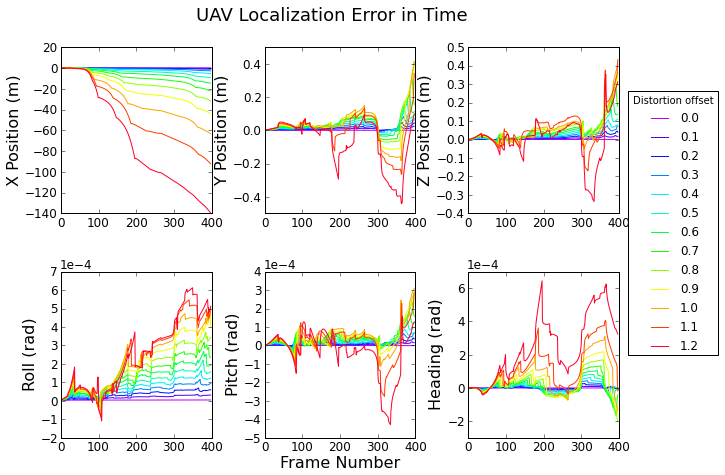
\includegraphics[width=14cm,keepaspectratio=true]{./Figures/SimulationFigures/Figure48.png}
  \caption{Diverging UAV localization errors for various lens
    distortion settings}
  \label{fig:simfig48}
\end{figure}

The landmark position error statistics are shown in Figure
\ref{fig:simfig45}. The position errors are also plotted against
landmark ground truth positions in Figure \ref{fig:simfig46}. The
landmark positions on the X axis show the most error. The mean error
reaches -140 meters with distortion offset at 120\%. The amount of
error is related to the landmarks' distance from the X axis which aligns
with the optical axis (Figure \ref{fig:simfig46}, subplots [1,2] and
[1,3]). The further the landmarks lay from the X axis, the bigger the
errors they suffer. Landmark positions on the Y and Z axes have less
mean error, but the standard deviation are bigger. Figure
\ref{fig:simfig46} subplots [2,2] and [3,3] show that the errors on the
Y (or Z) axis are loosely proportional to the landmark ground truth
coordinates on the Y (or Z) axis, where the amount of error in distortion
determines the slope of the line. The relation indicates that
landmarks lying around the sides of the image plane carry more
errors than landmarks at the center of the image on all axes. This is
exactly the kind of error that radial distortion corrects for.

\begin{figure}[h]% get rid of title and reposition x label
  \centering
  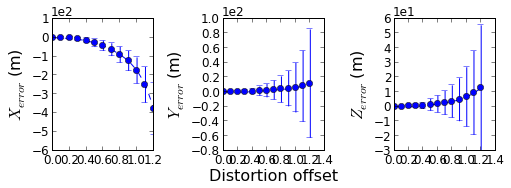
\includegraphics[width=10cm,keepaspectratio=true]{./Figures/SimulationFigures/Figure45.png}
  \caption{Landmark mapping error statistics with various lens
    distortion settings}
  \label{fig:simfig45}
\end{figure}

\begin{figure}[h] %get rid of the title. 
  \centering
  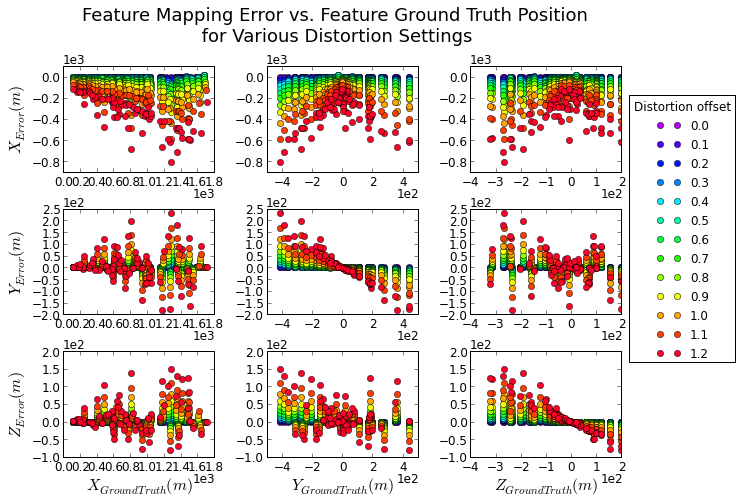
\includegraphics[width=13cm,keepaspectratio=true]{./Figures/SimulationFigures/Figure46.png}
  \caption{Landmark mapping errors versus landmark distance
    to optical axis with error in lens distortion}
  \label{fig:simfig46}
\end{figure}
\FloatBarrier

\subsection{Effect of Image Digitization}

It is well known that higher resolution sensors give more accuracy
to the estimates. To know how high a resolution is good enough for the
distance that this research is targeting at, a quantitative
analysis is necessary. Simulations were run with various image
resolution settings, and the results are shown in figure
\ref{fig:simfig50}.
\begin{figure}[h] 
  \centering
  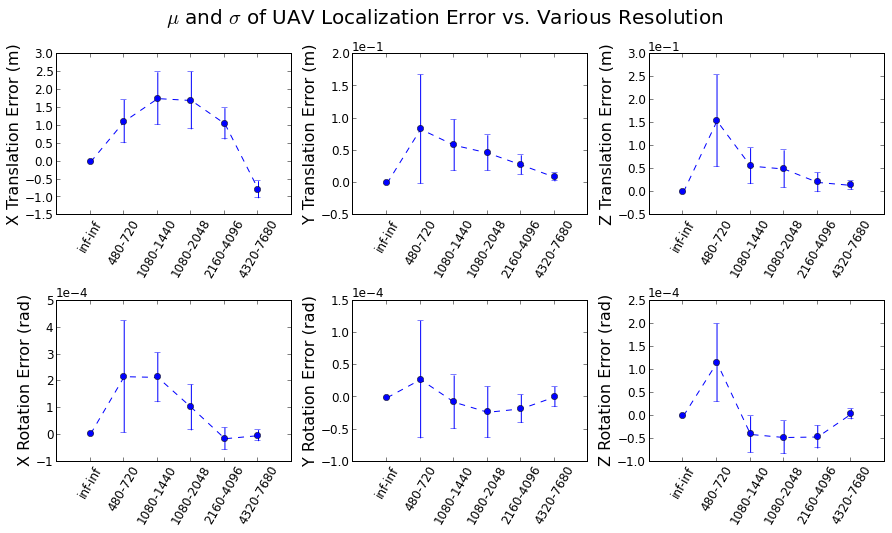
\includegraphics[width=10cm,keepaspectratio=true]{./Figures/SimulationFigures/Figure50.png}
  \caption{UAV localization error statistics for various image resolutions}
  \label{fig:simfig50}
\end{figure}

\begin{figure}[h] 
  \centering
  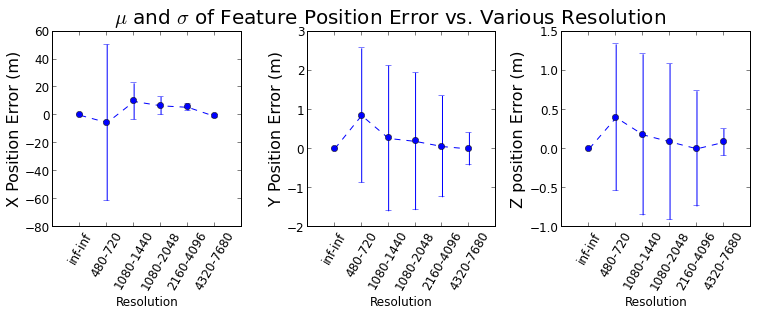
\includegraphics[width=10cm,keepaspectratio=true]{./Figures/SimulationFigures/Figure49.png}
  \caption{Landmark mapping error statistics for various image resolutions}
  \label{fig:simfig51}
\end{figure}

This test confirms that the higher resolution the image sensor has,
the more accuracy it will bring. The most significant error is seen
at resolution 480x720 where the landmark position errors on X are
+/- 150m. At 1080x1440, landmark position errors on the X axis are
greatly reduced to a few meters. For all other parameter estimates,
improvements at each increase of resolution are nearly linear.
This result suggests that, to achieve reasonably good accuracy for
obstacle detection, a sensor with resolution of 1080x1440 or higher is
preferred.


%%% Local Variables:
%%% mode: latex
%%% TeX-master: "thesis"
%%% End:
